% -*- LaTeX -*-

\sloppy

\title{\healpix IDL Facility User Guidelines}
\docid{outline\_earth} \section[outline\_earth]{ }
\label{idl:outline_earth}
\docrv{Version 1.0}
\author{Eric Hivon}
\abstract{This document describes the \healpix IDL facility \thedocid.}

\begin{facility}
{This IDL facility generates an outline of the Earth continents, coast lines, 
countries and/or rivers, at various resolution, 
which can then be overplotted onto \healpix maps using the 
\mylink{idl:mollview:outline}{outline} option of
\htmlref{cartview}{idl:cartview},
\htmlref{gnomview}{idl:gnomview},
\htmlref{mollview}{idl:mollview} or
\htmlref{orthview}{idl:orthview}.%
}
{src/idl/visu/outline\_earth.pro}
\end{facility}

\begin{IDLformat}
{\mylink{idl:outline_earth:geo}{geo} = 
OUTLINE\_EARTH([\mylink{idl:outline_earth:geo_in}{geo\_in}], [%
\mylink{idl:outline_earth:behavior}{BEHAVIOR=}, 
\mylink{idl:outline_earth:coasts}{/COASTS},
\mylink{idl:outline_earth:color}{COLOR=},
\mylink{idl:outline_earth:continents}{/CONTINENTS},
\mylink{idl:outline_earth:countries}{/COUNTRIES},
\mylink{idl:outline_earth:help}{/HELP},
\mylink{idl:outline_earth:hires}{HIRES=},
\mylink{idl:outline_earth:linestyle}{LINESTYLE=},
\mylink{idl:outline_earth:rivers}{/RIVERS},
\mylink{idl:outline_earth:thick}{THICK=}])}
\end{IDLformat}

\begin{qualifiers}
  \begin{qulist}{} %%%% NOTE the ``extra'' brace here %%%%
   \item[geo] \mytarget{idl:outline_earth:geo} output IDL structure
   \item[geo\_in] \mytarget{idl:outline_earth:geo_in} optional input IDL structure generated
by a previous call to \thedocid, which will be included into the output 
\mylink{idl:outline_earth:geo}{\texttt{geo}} (see \mylink{idl:outline_earth:example}{Example})
  \end{qulist}
\end{qualifiers}

\begin{keywords}
  \begin{kwlist}{} %%% extra brace
 \item[BEHAVIOR=] \mytarget{idl:outline_earth:behavior} either 'GDL', 'IDL' or absent: 
            changes the origin of the Earth data 
  (see \mylink{idl:outline_earth:description}{below})

 \item[/COASTS] \mytarget{idl:outline_earth:coasts} if set, adds coastlines, islands, and lakes information in \mylink{idl:outline_earth:geo}{\texttt{geo}} with the features 
\mylink{idl:outline_earth:color}{COLOR},
\mylink{idl:outline_earth:linestyle}{LINESTYLE} and
\mylink{idl:outline_earth:linestyle}{THICK}.

 \item[COLOR=] \mytarget{idl:outline_earth:color} scalar or 2-element array: color index to be given to geographical data in final plot in [0, 255]. See \mylink{idl:mollview:outline}{outline} of \htmlref{mollview}{idl:mollview} for details.

 \item[/CONTINENTS] \mytarget{idl:outline_earth:continents} if set, adds continental boundaries

 \item[/COUNTRIES] \mytarget{idl:outline_earth:countries} if set, adds political boundaries (as of 1993)

 \item[/HELP]      \mytarget{idl:outline_earth:help} if set, prints extended help

 \item[HIRES=] \mytarget{idl:outline_earth:hires}
	if set $>0$ use high resolution information (if it is available) 
              instead of default low resolution one.\\
              Either 0 or 1 (and more) in IDL mode;\\
              in {0,1,2,3,4} in GDL mode.\\
             Beware that Hires data are voluminous, longer to process
              and will result in large PNG or PDF files when plotted with eg mollview

 \item[LINESTYLE=] \mytarget{idl:outline_earth:linestyle} linestyle given to current geographical outline(s). \default{0}. See \mylink{idl:mollview:outline}{outline} of \htmlref{mollview}{idl:mollview} for details.

 \item[/RIVERS] \mytarget{idl:outline_earth:rivers} if set, adds rivers

 \item[THICK=] \mytarget{idl:outline_earth:thick} thickness of the geographical lines \default{1.0}.
See \mylink{idl:mollview:outline}{outline} of \htmlref{mollview}{idl:mollview} for details.

  \end{kwlist}
\end{keywords}  

\begin{codedescription}
{\thedocid\ \mytarget{idl:outline_earth:description}
 reads Earth data from disk (see below) and generates outlines of the Earth continents, coast lines, 
countries and/or rivers (in combination or separately), at various resolution, with a user-specified color, linestyle and thickness, which can then be overplotted onto \healpix maps using 
\htmlref{cartview}{idl:cartview},
\htmlref{gnomview}{idl:gnomview},
\htmlref{mollview}{idl:mollview} or
\htmlref{orthview}{idl:orthview}.
\\
-- If run under IDL (or if \mylink{idl:outline_earth:behavior}{BEHAVIOR}='IDL') 
  the Earth data are read from
  \texttt{\${IDL\_DIR}/resource/maps/*/*.*}
  with 'low' (\mylink{idl:outline_earth:hires}{HIRES}=0) and if available 'high' (\mylink{idl:outline_earth:hires}{HIRES}$\ge$1) resolution.
\\
-- If run under GDL (or if \mylink{idl:outline_earth:behavior}{BEHAVIOR}='GDL') the GSHHS data 
  (version 2.2 or more, available at 
  \url{https://www.ngdc.noaa.gov/mgg/shorelines/data/gshhg/latest}\texttt{/gshhg-bin-*.zip})
  are read from \texttt{\${GSHHS\_DATA\_DIR}/*.b}
  with \mylink{idl:outline_earth:hires}{HIRES}=0,1,2,3,4 standing for 'coarse', 'low', 'intermediate', 
  'high' and 'full' resolution respectively.\\
  In GDL mode, Coasts and Continents are degenerate.
\\
-- Under FL, \mylink{idl:outline_earth:behavior}{BEHAVIOR} must be set to either 'IDL' or 'GDL', 
  and the corresponding data must be available .
}
\end{codedescription}


\begin{related}
  \begin{sulist}{} %%%% NOTE the ``extra'' brace here %%%%
    \item[idl] version \idlversion or more is necessary to run \thedocid.
    \item[\htmlref{cartview}{idl:cartview}, \htmlref{gnomview}{idl:gnomview}]
    \item[\htmlref{mollview}{idl:mollview}, \htmlref{orthview}{idl:orthview}] 
visualization routines that overplot the Earth geographical outlines generated by \thedocid)
  \end{sulist}
\end{related}

%\newpage
%----------------------------------------------------------------------------
\begin{example}
{%
\mytarget{idl:outline_earth:example}%
\begin{tabular}{l} %%%% use this tabular format %%%%
geo = \thedocid(/continents,/hires,thick=0.8)\\% ; high res continents with thick lines\\
geo = \thedocid(geo, /rivers,      thick=0.1,col=20)\\% ; add low res rivers with thiner lines and a different color\\
\htmlref{mollview}{idl:mollview}, findgen(12), \$\\
\hspace{1em}  
\mylink{idl:mollview:outline}{outline}=geo, 
\mylink{idl:mollview:flip}{/flip}, 
\mylink{idl:mollview:coord}{coord=['C','C']}, \$\\
\hspace{1em}  min=-11,max=11,colt='planck1',/crop
\end{tabular}
}
{Creates a structure containing a thick-lined high-resolution continent outline, 
adds a thin-lined lower resolution rivers outline, in a different color, and then overplots the combination
on a Mollweide projection of a (simple) \healpix map
(see Fig.~\ref{fig:outline_earth}\latexhtml{ on page~\pageref{page:outline_earth}}{})
Note that since Earth data (generated in Celestial = eQuatorial coordinates) 
are usually shown with the longitude increasing from left to right 
(contrary to astronomical data), the \texttt{flip} keyword must be set in \texttt{mollview}.
}
%mollview, findgen(12),min=-11,max=11, outline=geo, /flip, coord=['C','C'],colt='planck1',/crop,png='/tmp/outline_earth.png',/prev,px=720
\end{example}

\begin{figure}[h!]
\latexhtml{%for latex
\centerline{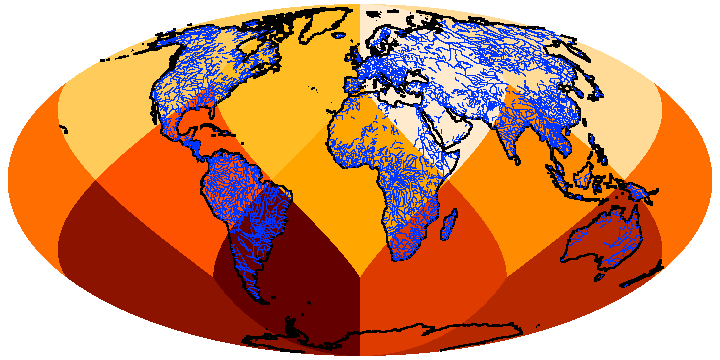
\includegraphics[width=0.99\textwidth]{fig/outline_earth}}
}{%for html
\centerline{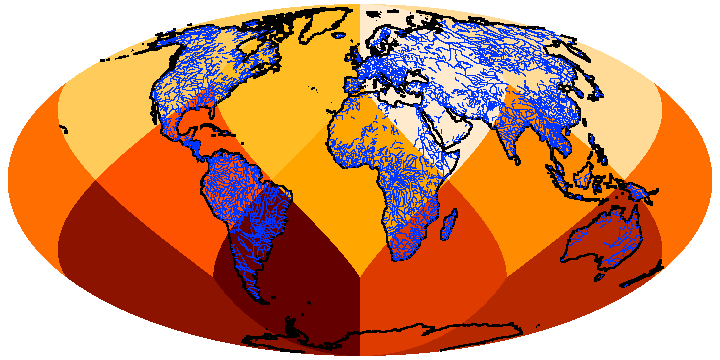
\includegraphics[width=520pt]{fig/outline_earth}{}}%rescaled for JPL web site -> ~720
}
\caption{%
\label{page:outline_earth}%
\label{fig:outline_earth}%
Illustration of the Earth outlines created by \latexhtml{\thedocid}{outline\_earth}.}
\end{figure}



%----------------------------------------------------------------------------
